\chapter{Simulation comparison \& evaluations}
In the previous chapter we have described our model, with the reactive concession stratgey. Here the reactive concession strategy is compared to nonreactive concession strategy. 

The nonreactive strategy used is as a base line.

Since the utility functions are private, utiliterian 

NASH solution:
product of the 

Nash bargening solution. 
convex optimilisaztion. Instead of product, max the log.
Convex optimization problem solving. 

The simaltation run is that of the Design

Mixbed water *2. The utility of water is a lot more important since the mixbed only has to clean a little.

Runnign the simulations:

for example. the solutions lay completely different. 


\citet{endriss2006monotonic} A concession should always be minimal with respect to the utility loss incurred by the agent making the concession.

\citet{endriss2006monotonic} Here some concession protocols are shown, \todo[explain monotonic multilateral concession protocols]{explain the multilateral concession protocols} however, since we are dealing with private information, this is not usefull. 


Agent anion and cation should form a front against the others, since they do not want water and mixbed is the only one wanting water.





















\section{Evaluation}


\section{Further research.}
At the moment, it seems as if the reactive concession strategy, as described in \citet{zheng2015automated} still has some difficulties. This can be clearly seen in \cref{fig:solution-mixbed-neut}. 
\begin{figure}[h]
	\centering
	\includegraphics[width=0.7\linewidth]{"img/solution mixbed neut"}
	\caption{The current search for a solution for the mixbed agent and the neut agent. They do not find a solution in the solution space.}
	\label{fig:solution-mixbed-neut}
\end{figure}

\begin{figure}[h]
	\centering
	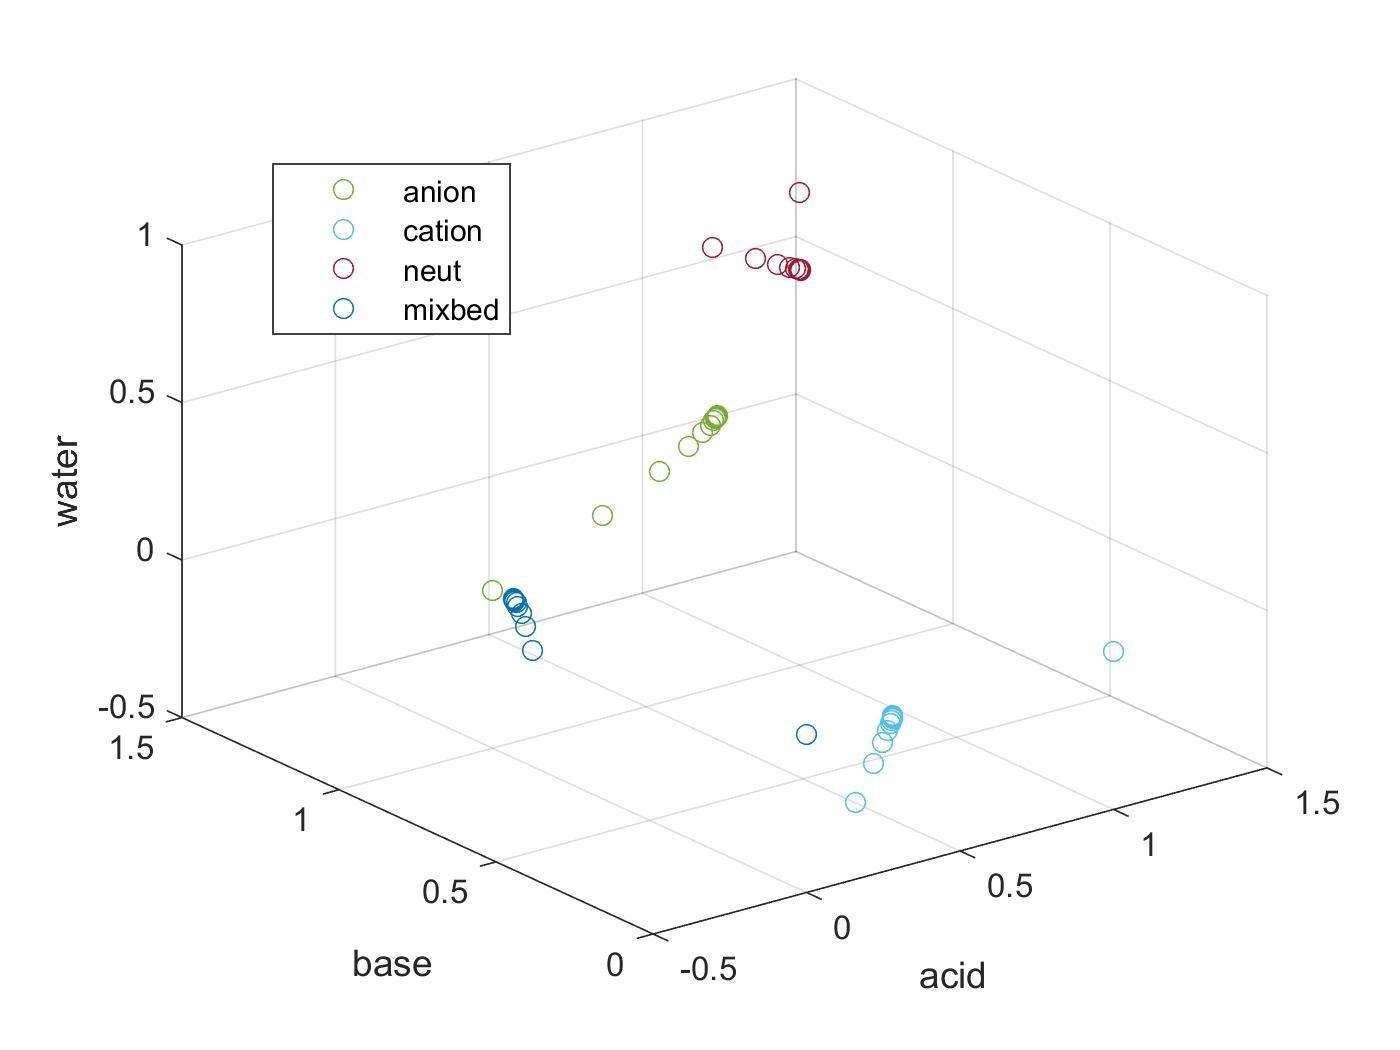
\includegraphics[width=0.7\linewidth]{img/scatter_of_proposals}
	\caption{A scatter plot of the proposals of the agents.}
	\label{fig:scatterofproposals}
\end{figure}


	

\subsection{Holonistic agents}

This structure is that of a holon as can be seen in figure~\cref{fig:holonexample}. As shown in the literature it is based on PROSA by \citet{van1998reference}.
\begin{figure}
	\centering
	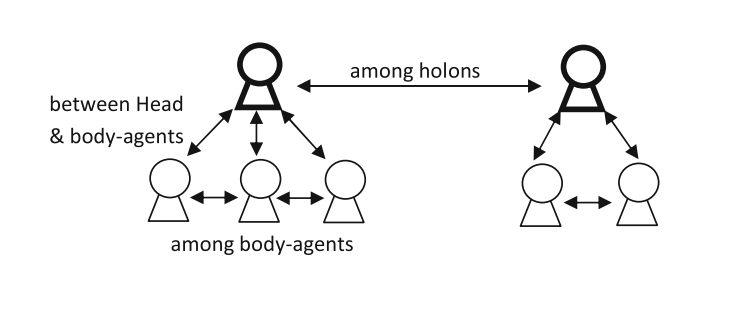
\includegraphics[width=0.7\linewidth]{img/holon_example}
	\caption{An example of the different negotiation between holons from \citet{beheshti2016negotiations}.}
	\label{fig:holonexample}
\end{figure}

The following facts and rules are part of the Anion.

\begin{enumerate}
	\item
	Knowledge of anion head about the sub-agents:
	\begin{itemize}
		\item {$\{A_1, ..., A_6\}$ can process $a$ amount of water}
		\item {$\{A_1, ..., A_6\}$ needs to be cleaned after $b$ water}
		\item {$\{A_1, ..., A_6\}$ has filtered $c$ amount of water}
		\item {$\{A_1, ..., A_6\}$ needs $d$ base to clean}
		\item {$\{A_1, ..., A_6\}$ needs $e$ time to clean}
	\end{itemize}
	\item
	Currently $x$ amount of water being filtered 
	\item
	Currently $Z \subseteq \{A_1, ..., A_6\}$ filter being used for water filtering
	\item
	Currently $Y \subseteq \{A_1, ..., A_6\}$ filter being used for cleaning
	\item
	Currently $w$ amount of base being used for cleaning
\end{enumerate}

\begin{figure}[h]
	
	\centering
	\begin{tikzpicture}
	
	\node[circle,draw,  minimum size=1cm] (A1) at  (0,0) {A$_1$};
	\node[circle,draw,  minimum size=1cm] (A2) at  (0,-1.5) {A$_2$};
	\node[circle,draw,  minimum size=1cm] (A3) at  (0,-3) {A$_3$};
	\node[circle,draw,  minimum size=1cm] (A4) at  (0,-4.5) {A$_4$};
	\node[circle,draw,  minimum size=1cm] (A5) at  (0,-6) {A$_5$};
	\node[circle,draw,  minimum size=1cm] (A6) at  (0,-7.5) {A$_6$};
	%\draw  (0,-2.5) ellipse (1 and 3.4);
	
	\node[ellipse,  draw, minimum height =9cm, minimum width = 2.5cm ] (A) at (0,-3.75) {Anion};
	
	\end{tikzpicture}
	\caption{Anion head and sub-agents}
	\label{fig:anion-head-sub}
	
\end{figure}


\subsection{Utility function}
\subsubsection{Reservation curve}

\begin{figure}
	\centering
	\begin{tikzpicture}[domain=0.15:4]
	%\draw[very thin,color=gray] (0.01,0.01) grid (3.9,3.9);
	\draw[->] (0.02,0) -- (4.2,0) node[below] {$Water$};
	\draw[->] (0,0.02) -- (0,4.2) node[left] {$Base$};% node[pos=0.25, left] {$200 m^3 / hr$};
	\draw[color=black] plot (\x,{0.07*exp(\x)}) node[left] {$R_A$};
	\end{tikzpicture}
	\label{fig:anionreservationfunction}
	\caption{The reservation function for the Anion filter: the more water is filtered and given, the more base it requires.}
\end{figure}

\todo[What to do if more water is required?]{Say we have a situation where water production is required. Reservation utility of mixbed to 0.1, rest to 0.3.
When is there no solution?}

\todo[further research]{Further research }

\todos
